\begin{figure*}[h]
    \centering
    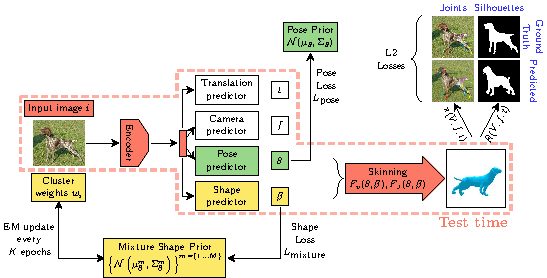
\includegraphics[width=\textwidth]{OllieFigs/system_overview_cr.pdf}
    \caption{Our method consists of (1) a deep CNN encoder which condenses the input image into a feature vector (2) a set of prediction heads which generate SMBLD parameters for shape $\beta$, pose $\theta$, camera focal length $f$ and translation $t$ (3) skinning functions $F_v$ and $F_J$ which construct the mesh from a set of parameters, and (4) loss functions which minimise the error between projected and ground truth joints and silhouettes. Finally, we incorporate a mixture shape prior (5) which regularises the predicted 3D shape and is iteratively updated during training using expectation maximisation. At test time, our system (1) condenses the input image, (2) generates the SMBLD parameters and (3) constructs the mesh.}
    \label{fig:sys_overview_train_sup}
\end{figure*}
    